\documentclass[12pt,a4paper]{article}

%\usepackage[square, comma, sort&compress]{natbib}
%\pagestyle{foot}
\textheight=255mm
\textwidth=175mm
\topmargin=-2.5cm
%\topmargin=0cm
\oddsidemargin=-1cm
%\parskip 3mm
%\setcounter{page}{1}
\newcommand{\thePIName}{萊斯利·蘭伯特}
\newcommand{\theProjectNo}{111WFD2610000}

\usepackage{epsfig}
\usepackage[nocompress]{cite}
\usepackage{amsmath}
\usepackage{amsfonts}
\usepackage{amssymb}
\usepackage{fancyhdr}
\usepackage{lastpage}
\usepackage{setspace}
\usepackage{enumerate}
\usepackage{hyperref}
\usepackage{xcolor}
\usepackage{url}

\onehalfspacing
\pagestyle{fancy}
\fancyhead{}
\fancyfoot{}
\renewcommand{\headrulewidth}{0pt}
\renewcommand{\footrulewidth}{0pt}
\newcommand\tab[1][1cm]{\hspace*{#1}}
\setlength{\headwidth}{\textwidth}

\lfoot{\footnotesize 表 CM03\tab[1cm]  計畫主持人 : {\thePIName} \tab[1cm] 申請條碼編號 : {\theProjectNo}}
\rfoot{\footnotesize 共~\pageref{LastPage}~頁\tab[0.5cm]第{~\thepage~}頁}

\usepackage{fontspec}
\usepackage[BoldFont]{xeCJK}
\setCJKmainfont{標楷體}
\XeTeXlinebreaklocale "zh"
\XeTeXlinebreakskip = 0pt plus 1pt

\newcommand{\enabstractname}{\textbf{\large Abstract}}
\newcommand{\cnabstractname}{\large 摘要}
\newenvironment{enabstract}{%
  \par\small\noindent
  \mbox{}\hfill{\bfseries \enabstractname}\hfill\mbox{}\par
  \vskip 3.5ex}{\par\vskip 5.5ex}
\newenvironment{cnabstract}{%
  \par\small
  \noindent\mbox{}\hfill{\bfseries \cnabstractname}\hfill\mbox{}\par
  \vskip 3.5ex}{\par\vskip 5.5ex}


% define a macro
%\def\texpsfig#1#2#3{\vbox{\kern #3\hbox{\special{psfile=#1}\kern #2}}\typeout{(#1)}}

\begin{document}
\newtheorem{thm}{Theorem}
\newtheorem{lem}{Lemma}
\newtheorem{cor}{Corollary}
\newtheorem{prop}{Proposition}
\newtheorem{conj}{Conjecture}
\newtheorem{definition}{Definition}
\input epsf   % load the epsf library

\baselineskip 7mm

\noindent
\textbf{\large  三、研究計畫內容(以中文或英文撰寫):}
\begin{description}
\small{
\itemsep-0.3em
\item[(一)]  研究計畫之背景。請詳述本研究計畫所要探討或解決的問題、重要性、預期影響性及國內外有關本計畫之研究情況、重要參考文獻之評述等。如為連續性計畫應說明上年度研究進度。
\item[(二)] 研究方法、進行步驟及執行進度。請分年列述:1.本計畫採用之研究方法與原因。2.預計可能遭遇之困難及解決途徑。3.重要儀器之配合使用情形。4.如為須赴國外或大陸地區研究,請詳述其必要性以及預期效益等。
\item[(三)] 預期完成之工作項目及成果。請分年列述:1.預期完成之工作項目。2.對於參與之工作人員,預期可獲之訓練。3.預期完成之研究成果(如期刊論文、研討會論文、專書、技術報告、專利或技術移轉等質與量之預期成果)。4.學術研究、國家發展及其他應用方面預期之貢獻。
\item[(四)] 整合型研究計畫說明。如為整合型研究計畫請就以上各點分別說明與其他子計畫之相關性。
}
\end{description}
\newpage

\begin{center}
{ \Huge \bfseries 科技部專題研究計畫 \LaTeX~template} \\[1cm]
\end{center}
\begin{cnabstract}\noindent\normalsize
LaTeX,是一種基於TeX的排版系統,由美國電腦科學家萊斯利·蘭伯特在20世紀80年代初期開發,利用這種格式系統的處理,即使使用者沒有排版和程式設計的知識也可以充分發揮由TeX所提供的強大功能,不必一一親自去設計或校對,能在幾天,甚至幾小時內生成很多具有書籍品質的印刷品。

\vskip 6.0ex
\noindent\textbf{關鍵字:}\LaTeX~template
\end{cnabstract}
\newpage

\begin{center}
{ \Huge \bfseries MOST Project \LaTeX~template} \\[1cm]
\end{center}
\begin{enabstract}\noindent\normalsize
\LaTeX is a high-quality typesetting system; it includes features designed for the production of technical and scientific documentation. \LaTeX is the de facto standard for the communication and publication of scientific documents. \LaTeX is available as free software.


\vskip 6.0ex
\noindent\textbf{Keywords:} \LaTeX~template
\end{enabstract}

\newpage
\section{Expected Research Results and Impacts}
\label{sec:expected_impacts}

\LaTeX is a high-quality typesetting system; it includes features designed for the production of technical and scientific documentation. \LaTeX is the de facto standard for the communication and publication of scientific documents. \LaTeX is available as free software.


\newpage
\section{Objective and Background}
\label{sec:objective}
\LaTeX is a high-quality typesetting system; it includes features designed for the production of technical and scientific documentation. \LaTeX is the de facto standard for the communication and publication of scientific documents. \LaTeX is available as free software.

\begin{figure}[t]
  \centering
  \centerline{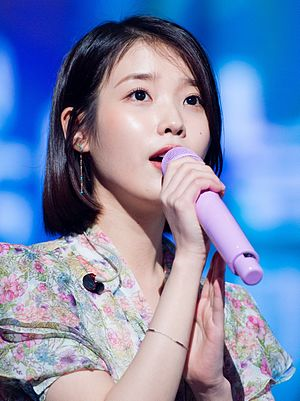
\includegraphics[width=8cm]{IU.jpg}}
  \caption{李知恩,藝名IU,是一名韓國創作歌手}
  \label{fig:fig1}
\end{figure}

\subsection{Background}
\label{sec:relatedwork}
\LaTeX is a high-quality typesetting system; it includes features designed for the production of technical and scientific documentation. \LaTeX is the de facto standard for the communication and publication of scientific documents. \LaTeX is available as free software.

\newpage
\section{Research Problems and Methods}
\label{sec:researchmethods}

\LaTeX is a high-quality typesetting system; it includes features designed for the production of technical and scientific documentation. \LaTeX is the de facto standard for the communication and publication of scientific documents. \LaTeX is available as free software.



% \subsection{The First Year Project}
% \label{sec:firstyear}



\subsection{The expected goals}
\LaTeX is a high-quality typesetting system; it includes features designed for the production of technical and scientific documentation. \LaTeX is the de facto standard for the communication and publication of scientific documents. \LaTeX is available as free software.
\begin{enumerate}[1)]
\item \LaTeX is a high-quality typesetting system.
\end{enumerate}


\subsection{Working tasks}
\LaTeX is a high-quality typesetting system; it includes features designed for the production of technical and scientific documentation. \LaTeX is the de facto standard for the communication and publication of scientific documents. \LaTeX is available as free software~\cite{ICDMW2021}.


\newpage
\label{LastPage}
\begingroup \small
\makeatletter
\renewcommand\@openbib@code{\itemsep\z@}
\makeatother
\bibliographystyle{ieeetr}
\bibliography{main}
\endgroup
\end{document}
